\documentclass{beamer}
\usepackage[spanish]{babel}
\usepackage[utf8]{inputenc}
\usepackage[pdftex]{graphicx}
\graphicspath{ {images/} }
\usetheme{metropolis}           % Use metropolis theme

\title{Linux para web developers}
\date{\today}
\author{Andrea Gómez}
\institute{Laboratoria}
\begin{document}
  \maketitle
  \section{Sistemas operativos}

  \begin{frame}{Sistema operativo}
    Es el principal programa que se ejecuta en toda computadora de propósito general y es el único programa que interactúa directamente con el hardware.
    \begin{figure}[ht!]
      \centering
      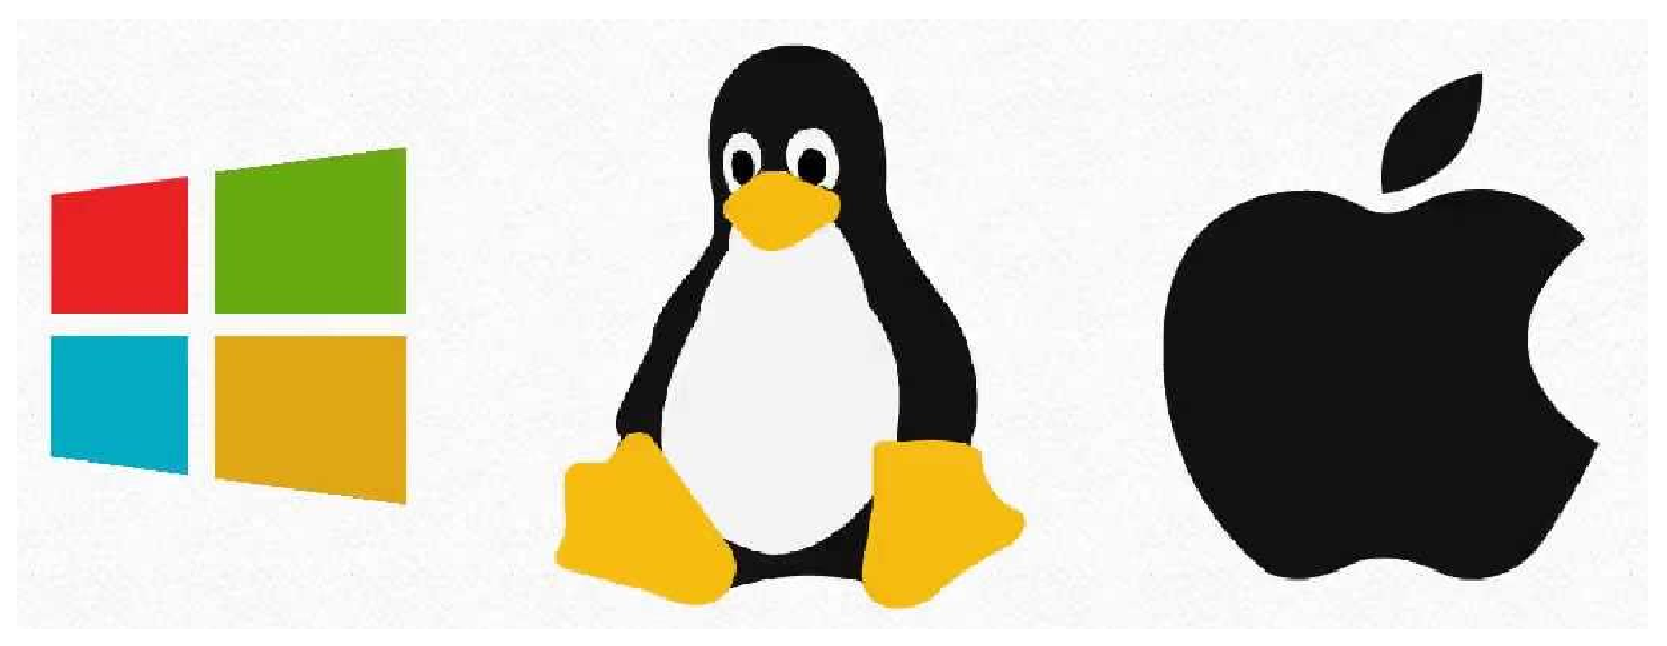
\includegraphics[width=50mm]{sistemasoperativos.eps}
    \end{figure}
  \end{frame}

  \begin{frame}{Funciones de un sistema operativo}
    \begin{enumerate}
    \item \textbf{Abstracción\\}
      {\small Los programas no se deben preocupar por detalles de acceso a hardware sino en resolver necesidades de usuarios.}
    \item \textbf{Administración de recursos\\}
      {\small Implementa políticas que asignan recursos a cada proceso.}
    \item \textbf{Aislamiento\\}
      {\small En un sistema multiusario y multitarea los usuarios y procesos no se deben preocupar por otros que estén usando el sistema.}
    \end{enumerate}
  \end{frame}

  \begin{frame}{El estándar POSIX}
    \begin{figure}[ht!]
      \centering
      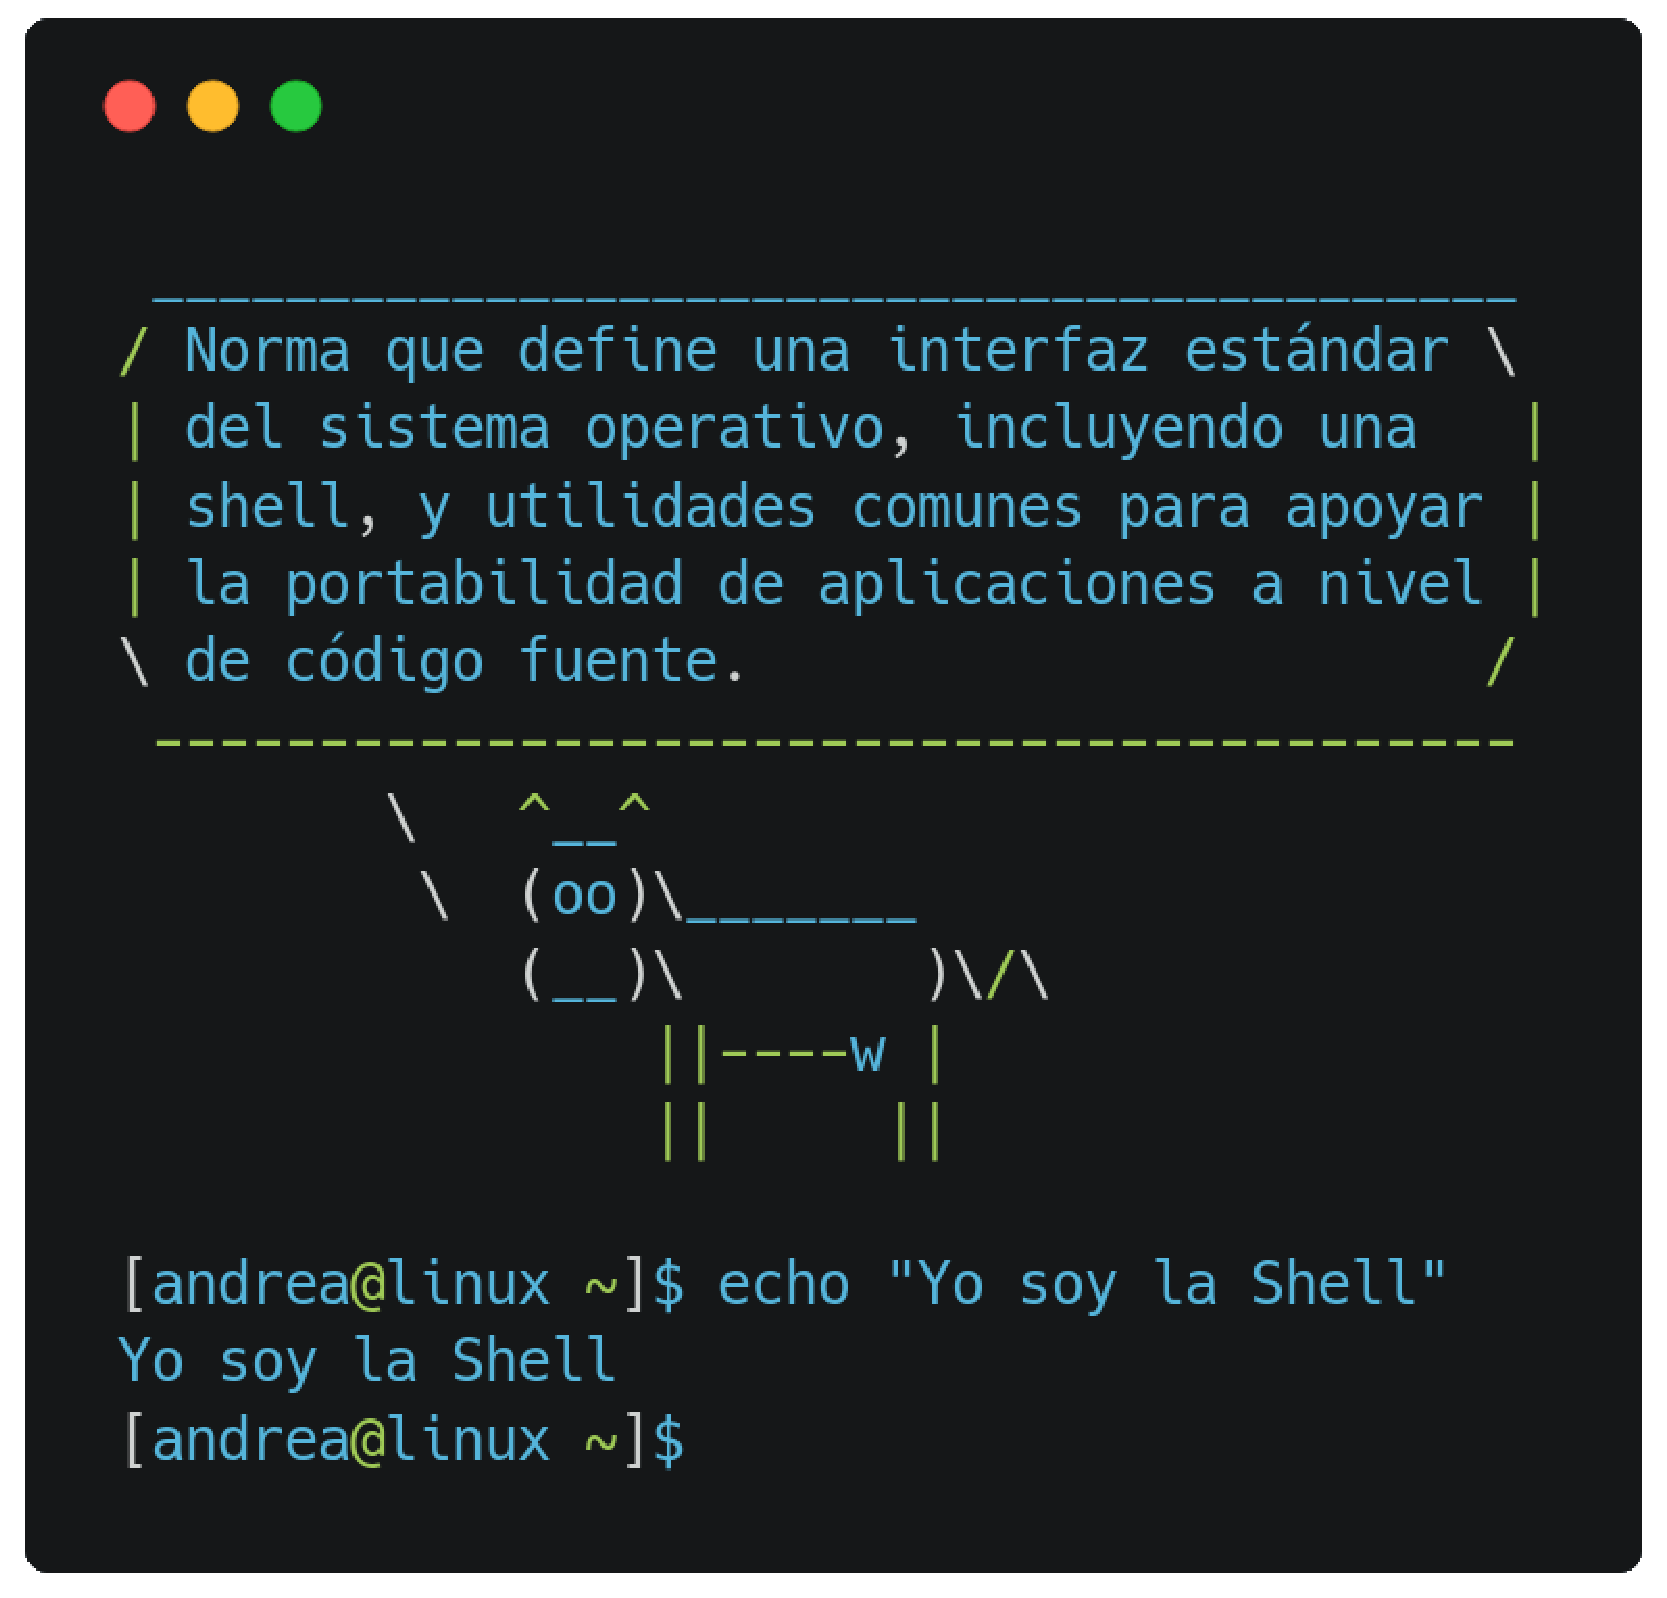
\includegraphics[height=80mm]{shell.eps}
    \end{figure}
  \end{frame}

  \begin{frame}{¿Quién usa Linux?}
    \begin{figure}[ht!]
      \centering
      
\includegraphics[width=110mm]{empresas.eps}
    \end{figure}
    \centering
    {\small Entre muchas otras empresas, organizaciones y personas.}
  \end{frame}

  \begin{frame}{¿Por qué usar Linux?}
    \item \textbf{Algunos beneficios de usar Linux:}
    \begin{columns}[T,onlytextwidth]
    \column{0.49\textwidth}
      \begin{itemize}
        \item Es gratuito y código abierto \item Estable y seguro \item Muy usado en servidores
      \end{itemize}

    \column{0.49\textwidth}
      \begin{itemize}
        \item Comunidad mundial de desarrollo \item Libre y personalizable \item Es divertido :)
        \end{itemize}
      \end{columns}
    \end{frame}

    \begin{frame}{Distribuciones de Linux}
      \item Una distribución de Linux es una versión de Linux creada para satisfacer
        necesidades específicas de sus usuarios.
        \begin{figure}[ht!]
          \centering
          
\includegraphics[width=90mm]{distros.eps}
        \end{figure}
    \end{frame}

    \begin{frame}{Fin de la presentación}
        \begin{figure}[ht!]
          \centering
          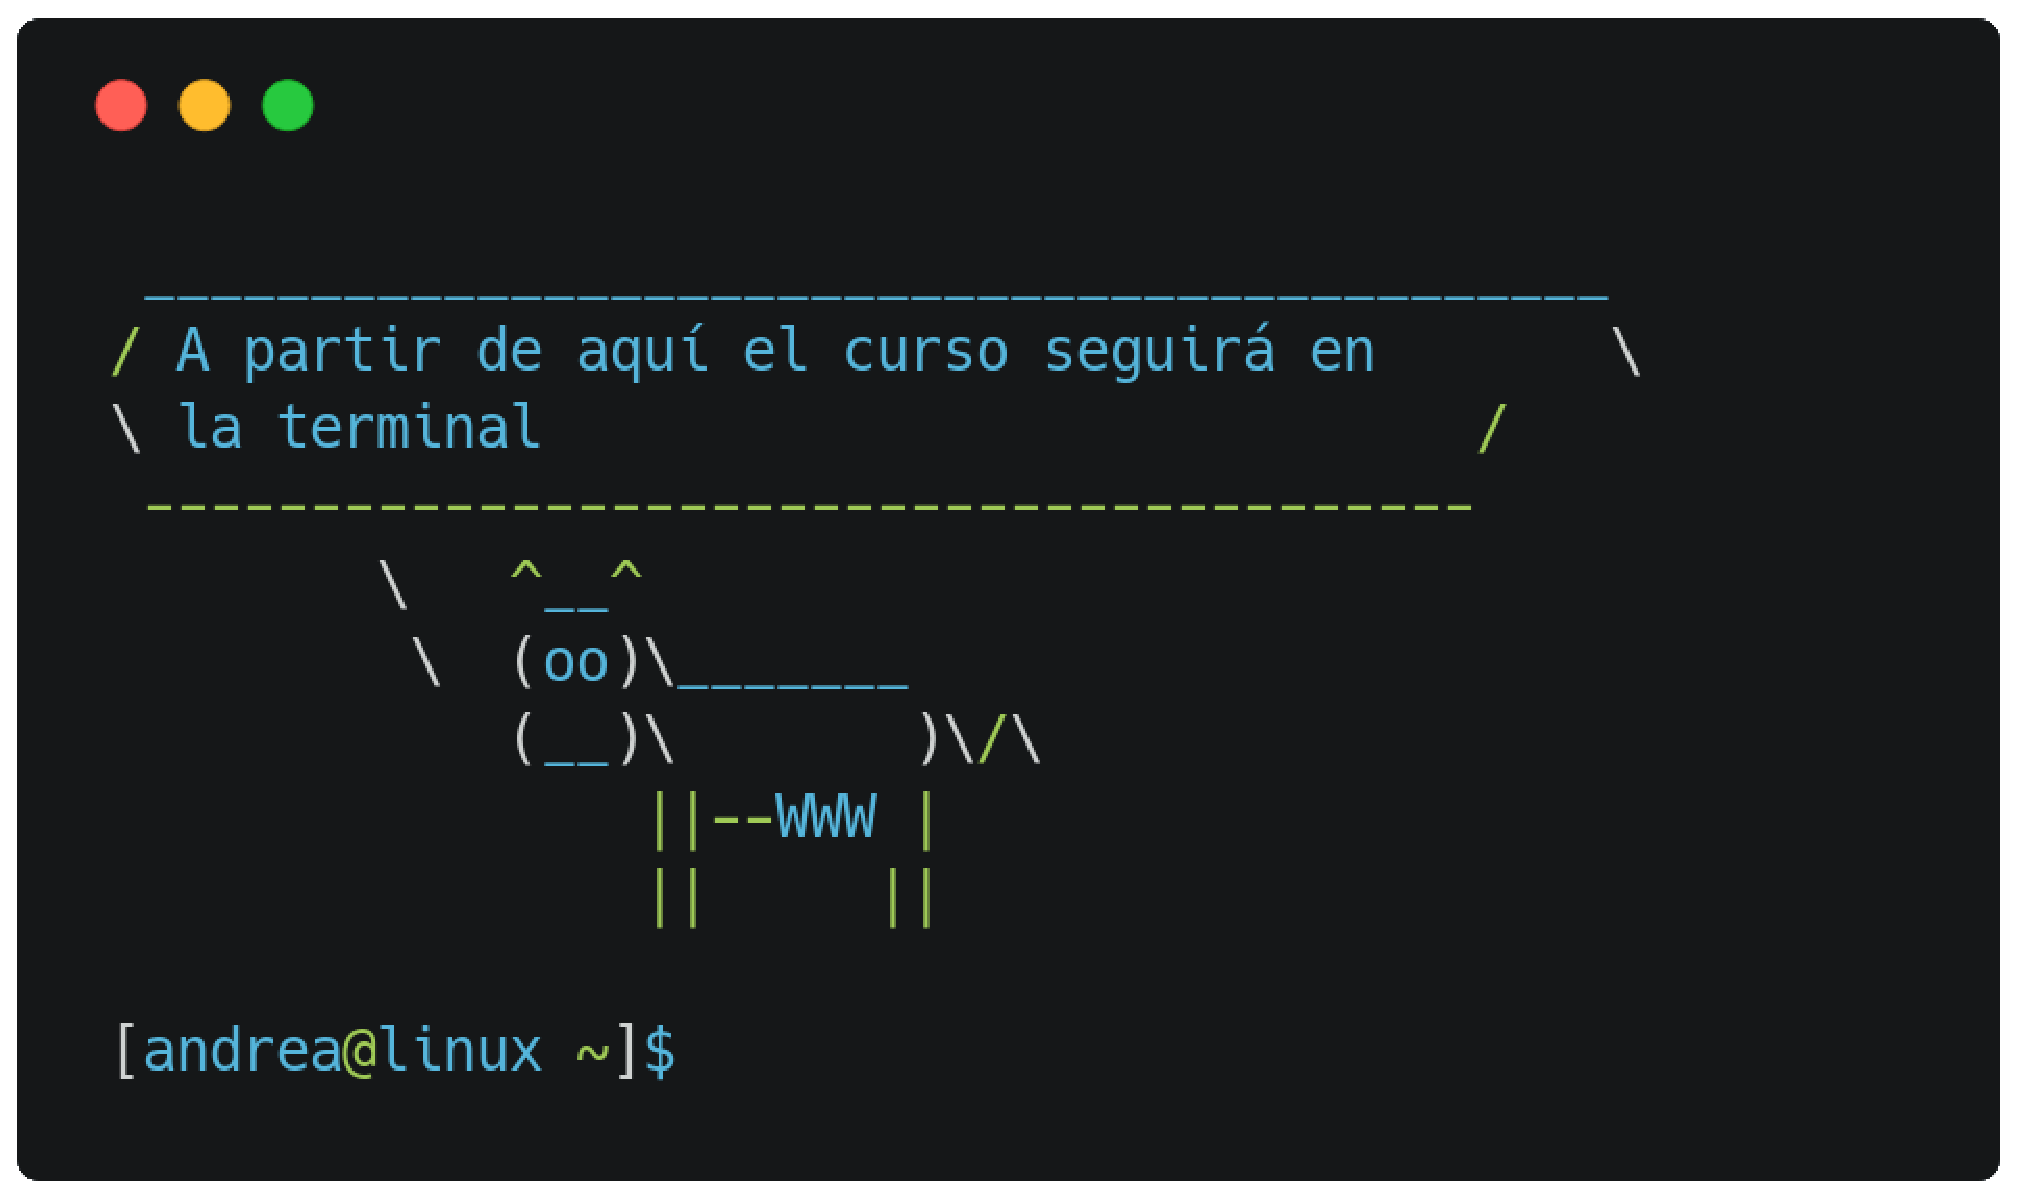
\includegraphics[width=90mm]{terminal.eps}
        \end{figure}
    \end{frame}  
\end{document}